\documentclass[tikz,border=5mm]{standalone}
\usepackage{tikz}
\usepackage{etoolbox}
\usetikzlibrary{positioning,matrix,backgrounds,calc}


\pgfdeclarelayer{background}
\pgfdeclarelayer{foreground}
\pgfsetlayers{background,main,foreground}

\definecolor{sindynullgray}{RGB}{200,200,200}
\definecolor{sindyforces}{RGB}{196,78,82}
\definecolor{sindynewton}{RGB}{85,168,104}
\definecolor{sindylagrange}{RGB}{129,114,179}

\newcommand{\lb}{[}
\newcommand{\rb}{]}

% Define the sindy component as a node style
\tikzset{
    sindy label/.style={font=\tiny, text=black,minimum height=0pt,inner sep =2pt,yshift=-4pt},
    sindy component text/.style={
        rectangle,
        minimum width=10pt,
        minimum height=1.5cm,
        rounded corners=5pt,
        fill=none,
        draw=none,
        inner sep=0pt,
        outer sep=2pt,
        align=center,
    },
    with label/.style={label={[sindy label]above:#1}},
    dots label/.style={
        rectangle,
        minimum width=0,
        minimum height=0,
        inner sep=-2cm,
        outer sep=0,
        rotate=#1
    },
    empty/.style={
        minimum width=0cm,
        minimum height=0.7cm,
        inner sep=0,
        outer sep=0,
        rounded corners=0
    },
    dots/.style={
        empty,
        minimum height=0cm,
        label={[dots label=#1]center:$\cdots$}
    }
}

%fill=none,rotate=\DOTANGLE,outer sep=-2cm,inner sep=-3cm,minimum height=0,minimum width=0

\begin{document}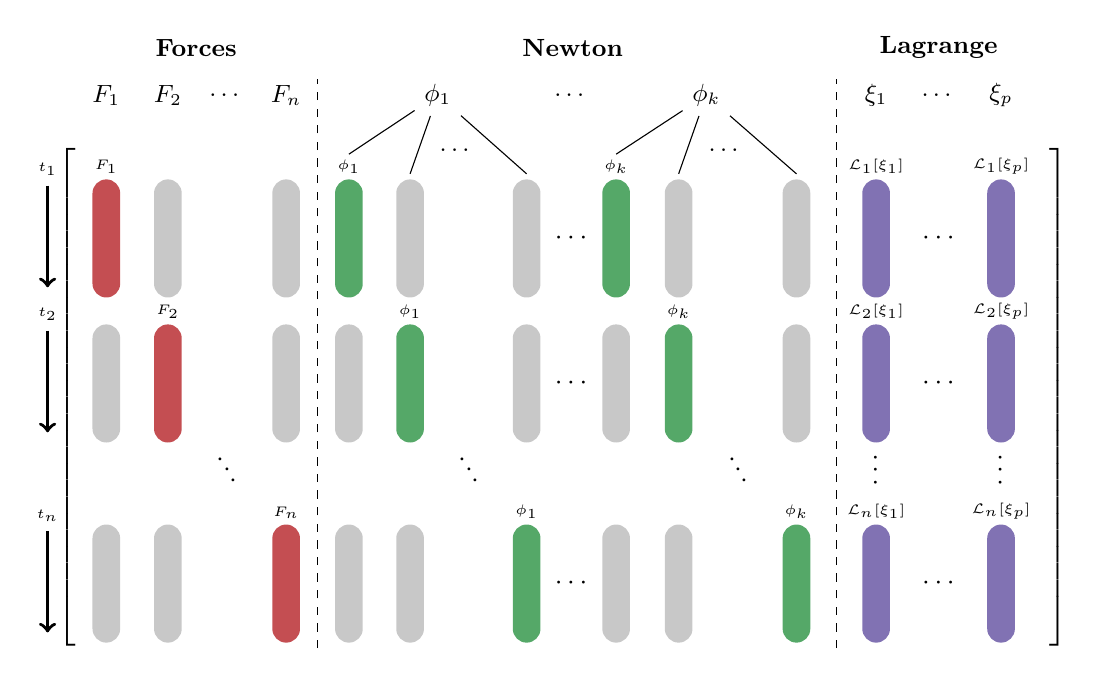
\begin{tikzpicture}
    \def\DIAGONALDOT{-60}
    %Create a matrix of nodes with automatic naming (m-row-column)
    \matrix[matrix of nodes,
            column sep=10pt, 
            row sep=0cm,
            nodes={sindy component text},
            left delimiter={[},
            right delimiter={]},
            nodes in empty cells
            ] (m) {
        |[fill=sindyforces,with label=$F_1$]| & |[fill=sindynullgray]| &  & |[fill=sindynullgray]| & |[fill=sindynewton,with label=$\phi_1$]| & |[fill=sindynullgray]| & & |[fill=sindynullgray]| & |[dots=0]| & |[fill=sindynewton,with label=$\phi_k$]| & |[fill=sindynullgray]| & & |[fill=sindynullgray]| & |[fill=sindylagrange,with label=$\mathcal{L}_1 \lb \xi_1 \rb$]| & |[dots=0]| & |[fill=sindylagrange,with label=$\mathcal{L}_1 \lb \xi_p \rb$]| \\
        |[fill=sindynullgray]| & |[fill=sindyforces,with label=$F_2$]| &  & |[fill=sindynullgray]| & |[fill=sindynullgray]| & |[fill=sindynewton,with label=$\phi_1$]| & & |[fill=sindynullgray]| & |[dots=0]| & |[fill=sindynullgray]| & |[fill=sindynewton,with label=$\phi_k$]| & & |[fill=sindynullgray]| & |[fill=sindylagrange,with label=$\mathcal{L}_2 \lb \xi_1 \rb$]| & |[dots=0]| & |[fill=sindylagrange,with label=$\mathcal{L}_2 \lb \xi_p \rb$]| \\
        |[empty]| & |[empty]| & |[dots=\DIAGONALDOT]| & |[empty]| & |[empty]| & |[empty]| & |[dots=\DIAGONALDOT]| & |[empty]| & |[empty]| & |[empty]| & |[empty]| & |[dots=\DIAGONALDOT]| & |[empty]| & |[dots=90]| & |[empty]| & |[dots=90]|\\
        |[fill=sindynullgray]| & |[fill=sindynullgray]| &  & |[fill=sindyforces,with label=$F_n$]| & |[fill=sindynullgray]| & |[fill=sindynullgray]| &  & |[fill=sindynewton,with label=$\phi_1$]| & |[dots=0]| & |[fill=sindynullgray]| & |[fill=sindynullgray]| & & |[fill=sindynewton,with label=$\phi_k$]| & |[fill=sindylagrange,with label=$\mathcal{L}_n \lb \xi_1 \rb$]| & |[dots=0]| & |[fill=sindylagrange,with label=$\mathcal{L}_n \lb \xi_p \rb$]| \\
        };

    \draw[dashed] ($(m-4-4.south east)!0.5!(m-4-5.south west)$) -- ($(m-1-4.north east)!0.5!(m-1-5.north west)$) -- ++(0,1.2cm);

    \draw[dashed] ($(m-4-13.south east)!0.5!(m-4-14.south west)$) -- ($(m-1-13.north east)!0.5!(m-1-14.north west)$) -- ++(0,1.2cm);

    \node at ($(m-1-1.north)!0.5!(m-1-4.north) + (0,1.6cm)$) {\small \textbf{Forces}};
    \node at ($(m-1-5.north)!0.5!(m-1-13.north) + (0,1.6cm)$) {\small \textbf{Newton}};
    \node at ($(m-1-14.north)!0.5!(m-1-16.north) + (0,1.6cm)$) {\small \textbf{Lagrange}};

    \node at ($(m-1-1.north) + (0,1cm)$) {\small $F_1$};
    \node at ($(m-1-2.north) + (0,1cm)$) {\small $F_2$};
    \node at ($(m-1-3.north) + (0,1cm)$) {\small \dots};
    \node at ($(m-1-4.north) + (0,1cm)$) {\small $F_n$};

    \node (phi1-label) at ($(m-1-5.north)!0.5!(m-1-8.north)  + (0,1cm)$) {\small $\phi_1$};
    \node at ($(m-1-8.north)!0.5!(m-1-10.north) + (0,1cm)$) {\small \dots};
    \node (phi3-label)at ($(m-1-10.north)!0.5!(m-1-13.north) + (0,1cm)$) {\small $\phi_k$};

    \draw (phi1-label) -- ($(m-1-5.north) + (0,0.25cm)$);
    \draw (phi1-label) -- (m-1-6.north);
    \draw (phi1-label) -- (m-1-8.north);
    \node at ($(m-1-6.north)!0.4!(m-1-8.north) + (0,0.3cm)$) {\small \dots};

    \draw (phi3-label) -- ($(m-1-10.north) + (0,0.25cm)$);
    \draw (phi3-label) -- (m-1-11.north);
    \draw (phi3-label) -- (m-1-13.north);
    \node at ($(m-1-11.north)!0.4!(m-1-13.north) + (0,0.3cm)$) {\small \dots};

    \node at ($(m-1-14.north) + (0,1cm)$) {\small $\xi_1$};
    \node at ($(m-1-14.north)!0.5!(m-1-16.north) + (0,1cm)$) {\small \dots};
    \node at ($(m-1-16.north) + (0,1cm)$) {\small $\xi_p$};

    \node[anchor=south] at ($(m-1-1.north west) + (-0.5cm,-0.15cm)$) {\tiny $t_1$};
    \draw[->,line width=1.25pt] ($(m-1-1.north west) + (-0.5cm,-0.15cm)$) -- ($(m-1-1.south west) + (-0.5cm,0.2cm)$);

    \node[anchor=south] at ($(m-2-1.north west) + (-0.5cm,-0.15cm)$) {\tiny $t_2$};
    \draw[->,line width=1.25pt] ($(m-2-1.north west) + (-0.5cm,-0.15cm)$) -- ($(m-2-1.south west) + (-0.5cm,0.2cm)$);

    \node[anchor=south] at ($(m-4-1.north west) + (-0.5cm,-0.15cm)$) {\tiny $t_n$};
    \draw[->,line width=1.25pt] ($(m-4-1.north west) + (-0.5cm,-0.15cm)$) -- ($(m-4-1.south west) + (-0.5cm,0.2cm)$);

    \end{tikzpicture}
\end{document}